\documentclass[11pt]{article}
\usepackage{amsmath}
\usepackage{amssymb}
\usepackage{graphicx}
\usepackage{geometry}[0.9in]
\usepackage{url}

\renewcommand{\vec}[1]{\boldsymbol{#1}}
\newcommand{\hvec}[1]{\hat{\vec{#1}}}

\title{Clarifications on scattering factors, scattering densities, and scattering intensity calculations.}
\author{Richard Kirian}
\date{\today}
\begin{document} 

\maketitle


\section{Atomic scattering density and atomic scattering factor}

Assuming monochromatic plane-wave illumination, far-field x-ray diffraction intensities under the first Born
approximation are equal to
\begin{align}\label{eqn:qrf}
I(\vec{q}) = J_0 \Delta \Omega r_e^2 P(\hvec{q}) \left| \sum_n^N f_n(\vec{q}) \exp(-i \vec{q}\cdot\vec{r}_n)\right|^2 = 
J_0 \Delta \Omega r_e^2 P(\hvec{q}) \left| f(\vec{q})\right|^2
\end{align}
where 
\begin{itemize}
\item[$J_0$] is the incident photon fluence (photons per area)
\item[$\Delta \Omega$] is the solid angle of the detector pixel (assumed
to be small)
\item[$r_e$] is the classical electron radius
\item[$P(\vec{q})$] is the polarization factor
\item[$f_n(\vec{q})$] is the $n$th atomic scattering factor
\item[$\vec{r}_n$] is the position vector of the $n$th atom
\item[$\vec{q}$] is the wavevector transfer
\item[$f(\vec{q})$] is the scattering factor of the entire object.
\end{itemize}
% We \emph{define} the complex scattering density $\rho(\vec{r})$ as
% \begin{align}\label{eqn:dft}
% I(\vec{q}) = J_0 \Delta \Omega r_e^2 P(\hvec{q})
% \left| \iiint_{-\infty}^\infty \rho(\vec{r}) \exp(-i \vec{q}\cdot\vec{r}) \; d^3r\right|^2 \; .
% \end{align}
For a rotationally symmetric atom\footnote{Most tabulations of scattering factors use a rotational symmetry approximation, and it is very rare to image with resolutions that can resolve internal atomic structure.} situated at the origin, the atomic scattering density is \emph{defined}
by the Fourier transform of $f_n(q)$\footnote{Appendix \ref{sec:3d1d} derives the relation between equations \ref{eqn:fn0} and \ref{eqn:form}.}
\begin{align}\label{eqn:fn0}
f_n(q)  &= \iiint_{-\infty}^\infty \rho_n(r) \exp(-i \vec{q}\cdot\vec{r}) \; d^3r \\
  &= \int_0^\infty \rho_n(r)   \frac{\sin(qr)}{qr}  4\pi r^2 dr \; . \label{eqn:form}
\end{align}
For an atom located at the position $\vec{r}_n$, the scattering factor takes on the phase shift
\begin{align}
f_n(\vec{q})  = \iiint_{-\infty}^\infty \rho_n(|\vec{r}-\vec{r}_n|) \exp(-i \vec{q}\cdot\vec{r}) d^3r = f_n(q)
\exp(-i \vec{q}\cdot\vec{r}_n)  \; .
\end{align}
The inverse Fourier transform of equation \ref{eqn:fn0} yields the atomic scattering density:
\begin{align}
\rho_n(r)  &= \frac{1}{8\pi^{3}} \int  f_n(q)  \exp(i \vec{q}\cdot\vec{r}) \; d^3q \\
&= \frac{1}{8\pi^{3}} \int_0^\infty f_n(q)   \frac{\sin(qr)}{qr}  4\pi q^2 dq \; . \label{rhor}
\end{align}
Atomic scattering factors are often approximated by a $q$-dependent ``atomic form factor'' $f_n^{(0)}(q)$  that is 
equal to the Fourier transform of the electronic wavefunction, along with a complex energy-dependent 
(but $q$-independent) ``anomalous dispersion correction'' $\Delta f_n(E) =  f_n'(E) + i f_n''(E)$:
\begin{align}
f_n(q) = f_n^{(0)}(q) + \Delta f_n(E) \; . %= f_0(q) + f'(E) + i f''(E)  \;.
\end{align}
Plugging these in we have
\begin{align}
\rho_n(r)  &= \frac{1}{8\pi^{3}} \iiint_{-\infty}^\infty  (f_n^{(0)}(q) + \Delta f_n(E))   \exp(i \vec{q}\cdot\vec{r}) \; d^3q \\
&=   \frac{1}{8\pi^{3}} \int_0^\infty f_n^{(0)}(q)    \frac{\sin(qr)}{qr}  4\pi q^2 dq + \delta(\vec{r}) \Delta f_n(E) \\
&=   \rho_n^{(0)}(r) + \delta(r) \Delta f_n(E)\; .
\end{align}
For an atom at position $\vec{r}_n$ we have
\begin{align}
\rho_n(\vec{r})  &= \rho_n^{(0)}(|\vec{r}-\vec{r}_n|) +  \delta(\vec{r}-\vec{r}_n) \Delta f_n(E)  \; ,
\end{align}
and the complete scattering density is the sum
\begin{align}
\rho(\vec{r})  &= \sum_n^N \rho_n(\vec{r}) \; .
\end{align}
With the above, we may compute the scattering amplitude of the atomic assembly by Fourier transforming the above:
\begin{align}
f(\vec{q})  &=  \iiint_{-\infty}^\infty \rho(\vec{r}) \exp(-i \vec{q}\cdot\vec{r}) \; d^3r\; .
\end{align}

\section{Numerical computations of $I(\vec{q})$}

Ultimately we wish to compute the intensities $I(\vec{q})$ for an ensemble of atoms.  We now see that there are two 
sensible options.  (1) We can directly compute the sum
\begin{align}
 \sum_n^N f_n(q) \exp(-i \vec{q}\cdot\vec{r}_n) \;,
\end{align}
which is a good option if there are not too many atoms.  Alternatively, (2) we first compute the sum
\begin{align}
\rho(\vec{r})  &= \sum_n^N \rho_n(\vec{r})
\end{align}
and Fourier transform the result.  This option is ideal in the event that there are a large number of atoms and
when a regular grid of $q$ samples is appropriate.  

numerical chores are the following:
\begin{enumerate}
\item Programmatically access the needed scattering factors $f_n^{(0)}$ and $\Delta f_n(E)$.
\item Deal with the fact that delta functions appear in the math and must be treated in an approximate way when 
sampling the scattering density $\rho_n(\vec{r})$ on a grid.
\item Do the transforms in equation \ref{rhor} numerically, or find lookup tables that already have $\rho(r)$.
\item Efficiently place the resulting $\rho_n(\vec{r})$ densities into a 3D grid.
\end{enumerate}

\section{Electron densities}

Below we develop the means to convert from form factors to densities.  However, atomic form factors usually derive from
calculated electron densities; converting from form factors to densities takes us full circle.  We should probably use
tabulated electron densities\cite{kogaAnalyticalHartreeFockElectron1996}.  The efforts described below
are for the purpose of having a corresponding set of structure factors in both real space and reciprocal
space.

\section{Cromer-Mann form factors}

The famous 1968 Cromer-Mann \cite{Cromer1968} table provides Hartree-Fock wavefunction approximations to the 
form factors of neutral atoms from He through Lw (along with some ions).  The table provides the $a_i$, $b_i$ and $c$ in the following expression:
\begin{align}
 f(\sin(\theta)/\lambda)=\sum_{i=1}^4 a_i \exp[-b_i \sin^2(\theta)/\lambda^2] + c \;.
\end{align}
Note that the usual $q$ is defined as $q=4\pi \sin(\theta)/\lambda$.  Now we take the Fourier transform
of the above to get the real-space scattering density:
\begin{align}
 \rho(r) &= \frac{1}{8\pi^3} \sum_{i=1}^4 a_i\int   \exp\left[-\frac{b_i}{16\pi^2} \vec{q}\cdot\vec{q}\right]\exp(i\vec{q}\cdot\vec{r})d^3q + c\int \exp(i\vec{q}\cdot\vec{r}) d^3q \\
 &=  \sum_{i=1}^4 a_i \prod_{j=1}^3\frac{1}{2\pi}\int   \exp\left[-\frac{b_i}{16\pi^2} q_j^2\right]\exp(iq_jr_j)dq_j + c\delta(\vec{r})
\end{align}
Note that the Fourier transform of a Gaussian is another Gaussian; from Abramowitz and Stegun \cite{Abramowitz1972} (eq. 7.4.6) the relation is
\begin{align}
 \int_{-\infty}^\infty e^{-ax^2}e^{-2\pi i kx}dx = \sqrt{\frac{\pi}{a}}e^{-\pi^2 k^2/a} \;,
\end{align}
which results in
\begin{align}
 \frac{1}{2\pi}\int   \exp\left[-\frac{b_i}{16\pi^2} q_j^2\right]\exp(iq_jr_j)dq_j = 2\sqrt{\frac{\pi}{b_i}}e^{-4\pi^2 q_j^2/b_i} \;.
\end{align}
Finally, 
\begin{align}
 \rho(r) =  \sum_{i=1}^4 a_i 8\left(\frac{\pi}{b_i}\right)^{3/2}e^{-12\pi^2 q_j^2/b_i} + c\delta(\vec{r}) \;.
\end{align}
Do note the delta function in the above.

\section{Hubbel form factors}

Hubbel {\itshape et al.} (1975)\cite{hubbellAtomicFormFactors1975} have provided tables of atomic form factors that are
still in widespread use today.  They provide atomic form factors $F(q,Z)$ (atomic number $Z$) that are defined exactly
as in equation \ref{eqn:form}.
The form factors $F(q,Z)$ are accessible programatically from the  \texttt{xraylib} library, which has a Python wrapper.

\section{Henke dispersion corrections} 

Henke {\itshape et al.}\cite{henkeXRayInteractionsPhotoabsorption1993} have compiled experimental dispersion corrections
that appear to be among the best available.  The Henke tables are largely meant for soft-x-ray work and as such they do
not include $q$-dependent scattering factors.
In the Henke {\itshape et al.}\cite{henkeXRayInteractionsPhotoabsorption1993} notation, the scattering factor is defined
as
\begin{align}
f=f_1+if_2=f_1(0)-\Delta f_0(\theta)+if_2(0)
\end{align}
and is related to the index of refraction by
\begin{align}
n_r = 1 - \delta -i\beta = 1 -\frac{r_0\lambda^2}{2\pi}\sum_q n_qf_q(0) \; .
\end{align}
The refractive index is always related to the electron density according to
\begin{align}
\rho =  \frac{2\pi}{\lambda^2 r_0 } \left( 1 - n_r \right) = \frac{2\pi}{\lambda^2 r_0 } \left( \delta + i \beta \right) 
\end{align}
The tabulated values of $f_1$ and $f_2$ are available in gzip format at the CXRO website
\url{http://henke.lbl.gov/optical_constants/asf.html}).  The \texttt{reborn} package provides programmatic access to
them.


\section{xraylib}

The \texttt{xraylib} library\cite{schoonjansXraylibLibraryXray2011,brunettiLibraryXrayMatter2004} provides access to the
atomic form factors  $F(x,Z)$  from Hubbel {\itshape et al.}\cite{hubbellAtomicFormFactors1975}.  They are accessed
through the function \texttt{FF\_Rayl(Z,q)} -- one can easily confirm correspondence with the Hubbel tables.  The
dispersion corrections are also accessible through the functions \texttt{Fi(Z,E)} and \texttt{Fii(Z,E)}, but there is
no mathematical definition of these functions in the \texttt{xraylib} publications, nor is there an explanation of where
they come from.   Empirically, the $f$ defined in the Henke tables is nearly equal to the quantity
$\texttt{FF\_Rayl(Z,q)} + \texttt{Fi(Z,E)} - i\; \texttt{Fii(Z,E)}$ that can be constructed from \texttt{xraylib}.  Note
the unconventional negative sign in front of the \texttt{Fii(Z,E)} term.  Figure \ref{fig:forms} shows plots comparing
the tabulated Henke tables and \texttt{xraylib} functions, which shows near equality, but the Henke tables seem to have
greater resolution near resonances.
\begin{figure}[htbp]
   \centering
   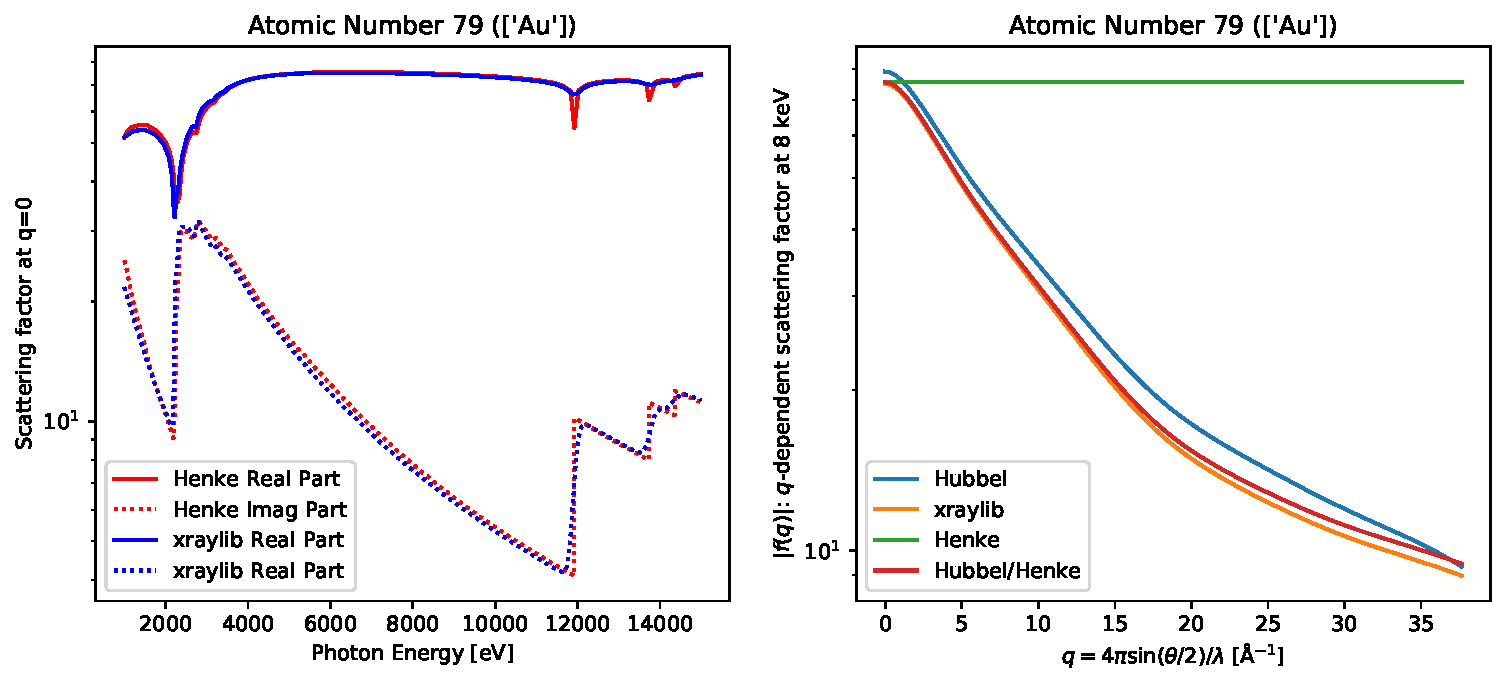
\includegraphics[width=\textwidth]{figures/formfactor_79.pdf} 
   \caption{Energy-dependent form factor in the forward scattering direction and the $Q$-dependent form factor.
   Comparison between Henke tables and \texttt{xraylib} for gold.  The plots were generated with the file
   \texttt{developer/rkirian/misc/scattering\_factors.py}.}
   \label{fig:forms}
\end{figure} 


\section{reborn}

These Henke scattering factors (at $q=0$) are returned as a single complex number $f$ from the function
\texttt{get\_scattering\_factors(Z,E)}, which is in the \texttt{reborn.simulate.atoms} sub-module.
\texttt{reborn} also has wrappers to the xraylib functions for convenience since they use different
units and they are not vectorized functions (hence they are very slow).  The combined Hubbel form
factors and Henke dispersion corrections may be accessed through the function
\texttt{reborn.simulate.atoms.hubbel\_henke\_atomic\_form\_factors}.




%%%%%%%%%%%%%%%%%%%%%%%%%%%%%%%%%%%%%%%%%%%%%%%%%%%%%%%%%%%%%%%%%%%%%%%%%
\section{Getting to the density}
%%%%%%%%%%%%%%%%%%%%%%%%%%%%%%%%%%%%%%%%%%%%%%%%%%%%%%%%%%%%%%%%%%%%%%%%%

We are provided with $f(q)$ from the Hubbel tables, along with the relation 
\begin{align}
  \rho(r) &= \frac{1}{2 \pi^2} \int_0^\infty     [q f(q)]  \frac{\sin(qr)}{r}dq  \;. \label{eqn:trans}
\end{align}
Note that we should treat the case of $r\rightarrow 0$ with care since we have have $\sin(qr)/r \rightarrow q$ in that limit.  Thus we have
a separate expression for $\rho(0)$:
\begin{align}
  \rho(0) &= \frac{1}{2 \pi^2} \int_0^\infty     [q^2 f(q)]  dq  \;. \label{eqn:trans0}
\end{align}
We aim to do this integral numerically.  We will discretize both $r$ and $q$ as follows:
\begin{align}
r_n &= n\Delta r \\
q_k &= k \Delta q
\end{align}
where $n$ and $k$ are integers.  The approximate integral is
\begin{align}
\rho(r_n) &\approx  \frac{1}{2 \pi^2 n\Delta r }\sum_{k=0}^{N-1}
[k \Delta q f(k \Delta q)]  \sin(k \Delta q n\Delta r) \Delta q \; .
\end{align}
We can do the above integral quickly if we use a Fast Fourier Transform (FFT) algorithm.  To see how this is done,
firstly note that the sin transform above is just the imaginary part of the Fourier Transform.  With some foresight, we
relate our gridpoints according to $\Delta q  = 2\pi / \Delta r N$, which gives us
\begin{align}
\rho(r_n) &\approx  \frac{1}{ \pi n\Delta r^2 }\text{Im}\left\{ \frac{1}{N}\sum_{k=0}^{N-1}
[k \Delta q f(k \Delta q)]  \exp\left(2\pi i \frac{ k  n}{N}\right) \right\} \; .
\end{align}
In numpy, the inverse FFT is defined in the following way:
\begin{align}\label{eqn:idft}
a_n = \text{FFT}^{-1}\left\{ A_k \right\}_n = \frac{1}{N}\sum_{k=0}^{N-1}A_k\exp\left(2\pi i \frac{nk}{N}\right)
\qquad n = 0,\ldots,N-1
\end{align}
If we define
\begin{align}
F_k &= k \Delta q F(k \Delta q) 
\end{align}
we arrive at the desired expression
\begin{align}\label{eqn:rhor}
\rho(n \Delta r) &\approx \frac{1}{\pi n \Delta r^2 } \text{Im} \left\{ \frac{1}{N}  \sum_{k=0}^{N-1}    F_k
\exp\left( 2\pi i \frac{nk}{ N} \right) \right\} = \frac{1}{\pi n \Delta r^2 } \text{Im}\left\{ \text{FFT}^{-1}
\left\{ F_k \right\}_n\right\} \; .
\end{align}
Equation \ref{eqn:rhor} has been tested and shown to agree in the case of the hydrogen atom, as shown in figure
\ref{fig:hydrogen} (the example script \texttt{scattering\_factors.py} that generated this plot is found in reborn).
However, there are some issues that remain at this time (1) the density near $r=0$ has a noticable error, and (2) there
are oscillatory artifacts that might be due to the truncation of $f(q)$.

\begin{figure}[htbp]
   \centering
   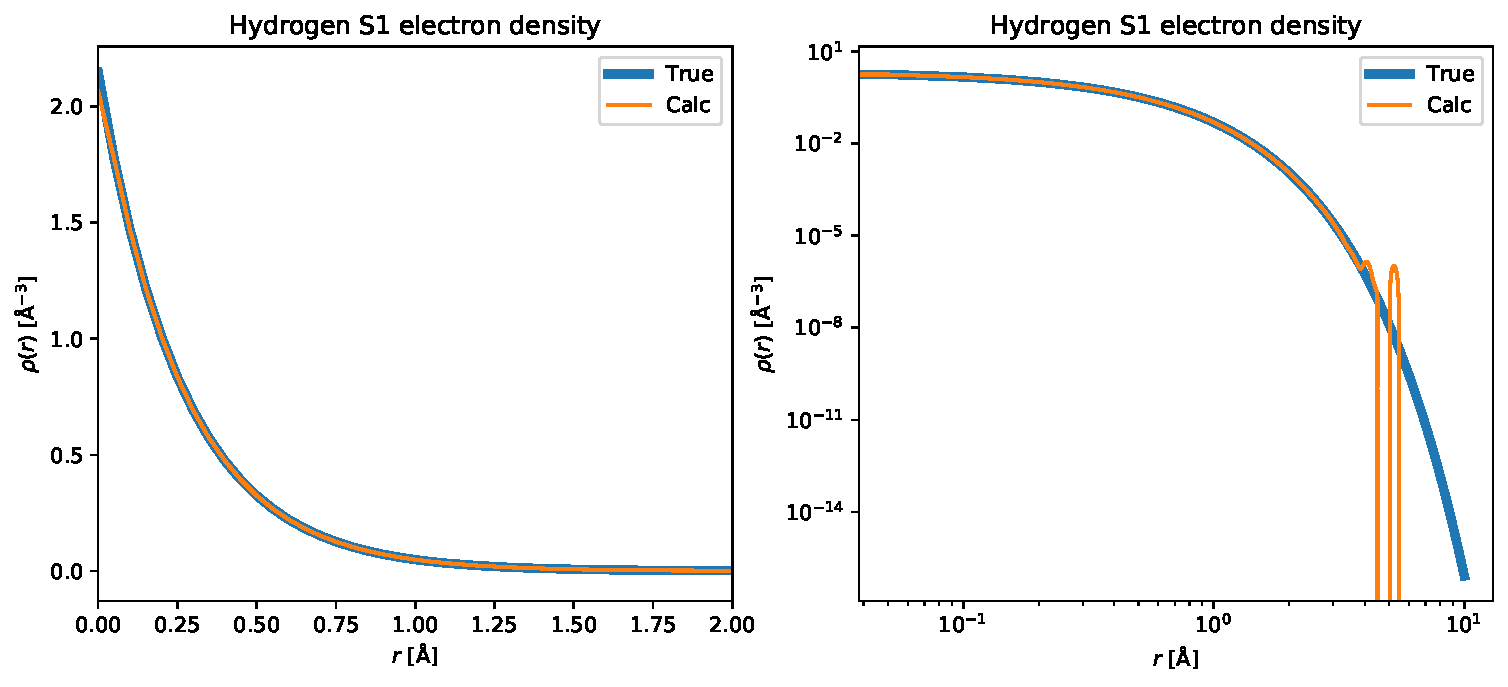
\includegraphics[width=\textwidth]{figures/hydrogen_density_1.pdf} 
   \caption{Hydrogen density calculated according to equation \ref{eqn:rhor}, compared against the analytic wavefunction
       $|\Psi(r)|^2=e^{-2 r/a_0}/\pi a_0^3$.}
   \label{fig:hydrogen}
\end{figure}

\section{Appendix}

\subsection{Fourier transform of rotationally symmetric object}
\label{sec:3d1d}

If we consider just a single atom situated at the origin, the atomic form factor is equal to
\begin{align}
 f(\vec{q})  = \int \rho(r) \exp(-i \vec{q}\cdot\vec{r}) \; d^3r \; .
\end{align}
Due to rotational symmetry, we are free to choose a convenient direction $\vec{q} = q \hvec{z}$ such that in the
spherical coordinate system we have $\vec{q}\cdot\vec{r} =  q r \cos\theta$.  Now we write down our Fourier transform with
reference only to the magnitudes $q$ and $r$:
\begin{align}
f(\vec{q})  &= \int_0^{2\pi} d\phi \int_0^\infty \rho(r) r^2 dr \int_0^\pi \sin\theta d\theta  \exp(-i q r \cos\theta)\\
&=2\pi \int_0^\infty \rho(r) r^2 dr \int_{-1}^1  d\cos\theta  \exp(-i q r \cos\theta)  \\
&=2\pi \int_0^\infty \rho(r) r^2 dr \frac{1}{-iqr}\int_{iqr}^{-iqr}  du  \exp(u)  \\
&=2\pi \int_0^\infty \rho(r) r^2 dr \frac{\exp(iqr) - \exp(-iqr)}{iqr}   \\
f(q) &= \int_0^\infty \rho(r)   \frac{\sin(qr)}{qr}  4\pi r^2 dr  
\end{align}

\newpage

\bibliography{\jobname}
\bibliographystyle{plain}

\end{document}
